\section{User Stories}
* how does HBM model building fit into research process?

\section{model building}
User Interface Design for HBM-builder 
The flow chart shown in figure \ref{HBM-build-process} represents the movement of a user through the process of building an HBM, or any graphical model for that matter.

\begin{figure}[!t]
  \centering
  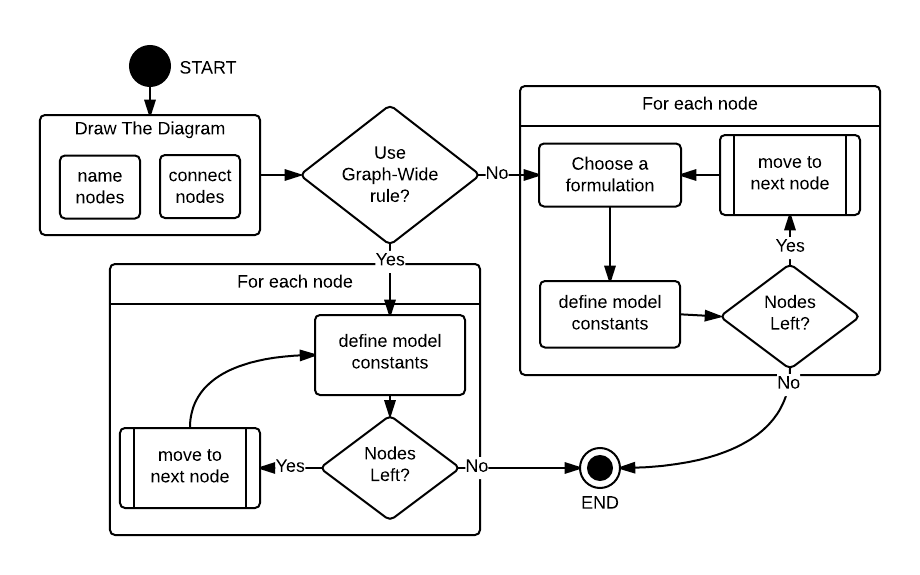
\includegraphics[width=0.9\columnwidth]{img/HBM-build-process}
  \caption{Flow chart depicting the process of building a graphical HBM.}
  \label{HBM-build-process}
\end{figure}

It is important to note that the process of building is pseudo-linear; users will likely want to jump back to an arbitrary point in the process and as the model takes shape. 
As the user moves through the process, they will re-assess the meaning of variables and connections and their model will solidify. 
UI for an HBM-building tool should enable easy backtracking and should work to provide feedback on the characteristics of the model early. 
The first iteration of the behaviorSim Model-Builder (see figure \ref{model-builder-v1}) took a step-wise approach to this task, which made backtracking difficult.

% [TODO picture of Model-Builder v0.1] 
\begin{figure}[!t]
  \centering
  1 
  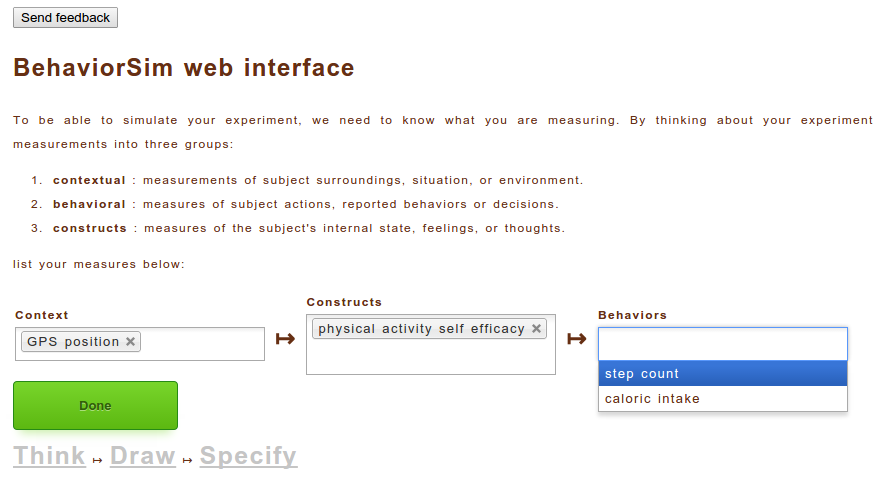
\includegraphics[width=0.9\columnwidth]{img/v1-think}
  \rule{\columnwidth}{0.4pt}
  2
  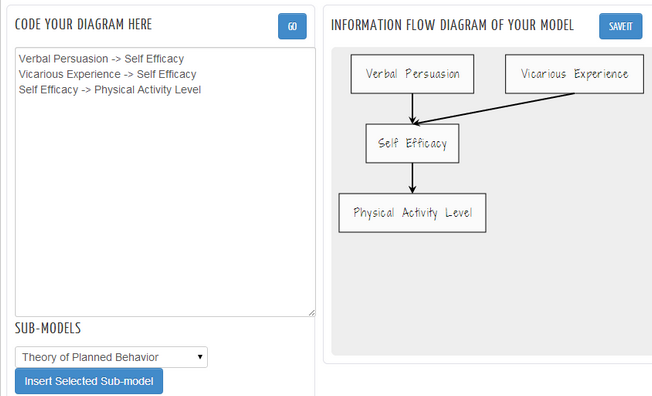
\includegraphics[width=0.9\columnwidth]{img/v1-draw}
  \rule{\columnwidth}{0.4pt}
  3
  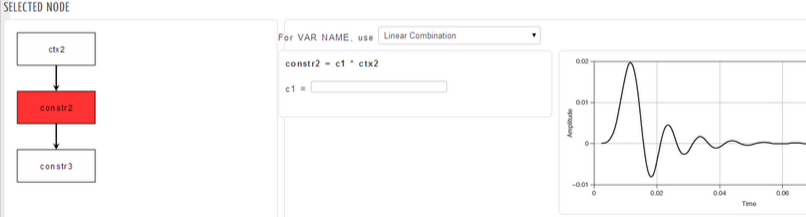
\includegraphics[width=0.9\columnwidth]{img/v1-specify}  
  \caption{behaviorSim Model Builder v0.1.x separated model-building into three separate stages: 1) think, 2) draw, 3) specify.}
  \label{model-builder-v1}
\end{figure}

A think-aloud assessment of this first version performed by four domain experts showed that in this design users have difficulty understanding how earlier choices related to later results, and feel constrained by previous choices rather than backtracking to revise the model.

The second generation of the Model Builder Tool presents a guided process which takes place within a single-page application. 
In this way, users can see how choices influence the model in real-time, and thus can iterate on their design much sooner.

While keeping the non-linearity of this process in mind, we will now walk through the diagram and address design considerations for each part of the process.

\subsection{Draw the Diagram}
This task involves the creation and connecting of all nodes in the diagram. 
Nodes and their connections should be primarily based in theory, so a user should be able to build a first draft of their model with little feedback. 
Once the formulas for each node have been specified, however, it is likely that the user will want to return to this step and reassess the network. 
Several paradigms diagram-drawing have been well tested, but there are essentially two prevailing options:
1) drag-and-drop node creation with drag-to-connect edges, and 2) textual ``diagram specification language''.

\subsubsection{drag-and-connect}
pros:
\begin{enumerate}
  \item{easy and intuitive to use}
\end{enumerate}
cons:
\begin{enumerate}
 \item can be difficult to position nodes to reduce edge overlap
 \item users often distracted trying to make graph "pretty"
 \item requires constant switching between mouse and keyboard2
\end{enumerate}

\subsubsection{Diagram Specification Language}
pros:
\begin{enumerate}
 \item can be much faster than mouse-based
 \item searching/finding nodes for modification is as easy as textual search
\end{enumerate}

cons:
\begin{enumerate}
 \item parsing errors can be a source of confusion
 \item user must learn the markup "language"
\end{enumerate}

\subsection{Use Graph-Wide Rule?}
This choice can come before or after the initial drawing of the graph, since it is likely the user has a graph-wide assumption in mind when starting the process. 
This choice determines whether or not the interface for specifying nodes individually is shown, so it is logical to think of the "none", "node-specific", or "node-unique" option as one of the choices available here. 

As an example, some graph-wide rules which may be implemented include:
\begin{enumerate}
  \item Probabilistic Graphical Network
  \item Linear Sum
  \item Fluid-Flow Analogy / Differential Equation Formulation (1st order and 2nd order)
\end{enumerate}

If a graph-wide rule is set, the formulation section for each node should show as locked to the rule's respective formulation. 
Editing an individual node's formulation will disable the graph-wide rule, and should require confirmation from the user. 

The interface for choosing one of these rules may be as simple as a select-option box or may include a detailed rule description and example. 

An additional feature which may be useful is to allow for user-defined graph-wide rules. 
In this case, users might choose "create new rule" and an interface to allow users to edit and save graph-wide rules is needed.

\subsection{For Each Node}

Items encapsulated by the "for each node" swim-lanes must be executed for each node in the graph. 
The graph-wide-rule-yes case differs from the graph-wide-rule-no case only in that the graph-wide-rule-no case requires the additional step of setting the formulation at each node.

\subsection{Choose a Formulation}
This item is identical to the graph-wide rule choice, except that it applies only to a single node. Similar design considerations apply, and user-defined choice is even more important at this scale.

\subsection{Define Model Constants}
The general solution of an HBM does not require definition of the constants, but a simulation cannot be run until some numerical value is assumed. 
These constants often have theoretical significance in that they often have meaningful influence upon system behavior. 
Scaling-coefficients, for instance allow for relative weighting of each inflow. 
Similarly, the coefficients of a dynamical equation define how quickly variables react to a change "upstream". 

UI for setting these constants could be as simple as a numerical input for each coefficient's name, but additional model details provided here may be of great benefit to the model designer. 

Firstly, UI should include equation-specific descriptions of the constants whenever possible. This means that a separate UI for each formulation type is necessary. 

Secondly, adjustment of coefficients would ideally show changes in the dynamics of a node's value in real-time. 
This can take the form of a time-series chart of the selected node's numerical value over time along with (editable) time-series for the inflows. 
Adjustment of these inflow series may also take a number of different forms. 

Thirdly, model creators may want to set these coefficients in three different ways: 
\subsubsection{1) Set the coefficient value to a constant}
All simulations derived from this general solution will have this exact value.

\subsubsection{2) Set a probability distribution for the coefficient}
Simulations derived from this general solution will select a numerical value based on the given distribution. 
This distribution may be learned from a training dataset, or bounds may be set for later training. 

\subsubsection{3) Leave the variable unbounded and assume a flat probability distribution}
This selection is identical to option 2 with a flat distribution from -infinity to +infinity.


These different ways of defining coefficients in a HBM become very important when it is time to run simulations and compare model results to real data. 

Lastly, model creators may want to use a measured value to set the value of these coefficients. In this way, one measured input (in real life), such as big-5 personality type, can be used to set the value of multiple coefficients across different variables in the model.

% Designing UI for the model-constant-defining process is complex enough to warrant it's own article, which I will write later and link to here(TODO).

\subsection{Nodes Left?}
%This is the most simple element of the flowchart. 
No if there are un-specified nodes remaining, yes if all are complete. 
It should be left to the user to confirm model-completeness, however, since a great deal of model-tweaking is likely now that simulation results can be displayed.

\subsection{Next Node}
Progression downstream through the model should be relatively straightforward in the case of tree-like models, but feedback loops can cause issues here. 
Perhaps the best paradigm here is to progress as naturally as possible, but allow the user to over-ride and select any node. 
This interaction mode is needed to allow for later model-tweaking anyway. 

The behaviorSim Model Builder v0.2 currently does not include significant enough indicator of node "completeness", so that the user is sometimes unsure when they should feel free to move to the next node.
